\documentclass[letterpaper,11pt]{article}

\usepackage[utf8]{inputenc}
\usepackage[spanish,mexico]{babel}
\usepackage{graphicx}
\usepackage{amsmath}
\usepackage{amsthm}
\usepackage{svg}
\usepackage{amsfonts}
\usepackage{subcaption}
\usepackage[hmargin=1in, vmargin=1in]{geometry}
\usepackage{fancyhdr}
\pagestyle{fancy}
\usepackage{tasks}
\lhead{\ExiCarrera}
\chead{\ExiMateria}
\rhead{\ExiParcial}
\cfoot{\ExiEscuela}
\renewcommand{\headrulewidth}{0.4pt}
\renewcommand{\footrulewidth}{0.4pt}

\providecommand{\abs}[1]{\lvert#1\rvert}
\providecommand{\norm}[1]{\lVert#1\rVert}

\newcommand{\informacion}[1]{
\begin{center}
\fbox{\fbox{\parbox{\textwidth}{{\footnotesize#1}}}}
\end{center}
\vspace{5mm}}
\newcommand{\datos}{\makebox[0.7\textwidth]{Nombre:~\hrulefill} Fecha:~\hrulefill}
\newcommand{\pregunta}[2]{\item{#2}~{(#1 puntos)}\\ \vspace{5mm}						       
			{\bf Solución}}														  
\newcommand{\ExiCarrera}{Matemáticas para las Ciencias II.}											 
\newcommand{\ExiMateria}{\textbf{Proyecto II}}														
\newcommand{\ExiParcial}{Entrega: Viernes 20 de Marzo}														  
\newcommand{\ExiEscuela}{\textbf{Facultad de Ciencias, UNAM}}	                		    
\begin{document}
\setlength{\unitlength}{1cm}
\thispagestyle{empty}
\begin{picture}(18,4)
\put(-0.5,1.2){
\includegraphics[scale=.25]{unam1.png}}
\put(13.5,1){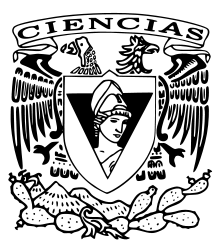
\includegraphics[scale=.35]{fciencias1.png}}
\end{picture}

\begin{center}
\vspace{-134pt}
\textbf{\large Estructuras de Datos}\\[0.2cm]
\textbf{ Semestre 2020-2}\\[0.2cm]
Prof. Alejandro Hernández Mora\\[0.2cm]
Ayud. Pablo Camacho González  \\ [0.2cm]
Ayud. Lab. Luis Manuel Martínez Dámaso   \\ [0.2cm]
\rule{17cm}{0.3mm}\\
\textbf{Tarea 1}\\
Kevin Ariel Merino Peña\footnote{317031326}\\
Armando Abraham Aquino Chapa\footnote{317058163}\\
\end{center}
\vspace{-10pt}
\rule{17cm}{0.3mm}
\begin{flushright}
\vspace{-3pt}
\end{flushright}

\noindent Durante la ejecución del programa siga las siguientes instrucciones

\section*{Instrucciones}

\begin{enumerate}

\item Para ejecutar el programa posicionarse en el metodo main y compilar con todas las clases necesarias.

\item La ruta por omision del archivo txt es \texttt{src/alumnos.txt}

\item En la primera ejecución, luego de posicionarse en la carpeta src (dentro de su terminal), debe seleccionar la opción 1, para pedir que lea un nuevo archivo de texto y la ruta debe ser: alumnos.txt
\end{enumerate}








\end{document}
